\documentclass{article}
\usepackage[top=0.5in, bottom=0.5in, left=1.25in, right=1.25in]{geometry}

\usepackage{amsmath, array, enumerate, tikz, bm, pgfplots, tcolorbox, graphicx, venndiagram, color, colortbl}
\pgfplotsset{compat = newest}
\usepgfplotslibrary{statistics}
\usepackage{pgf-pie}
\renewcommand{\familydefault}{\sfdefault}
\raggedright
\pagestyle{empty}

\newcounter{example}[section]
\newenvironment{example}[1][]{\refstepcounter{example}\par\medskip
   {\color{red}\textbf{Example~\theexample. #1}}}{\medskip}

\begin{document}

\section*{Qualitative Graphs}

\begin{tcolorbox}[colframe=orange!70!white, coltitle=black, title=\textbf{Summary}]
\begin{enumerate}
    \item Qualitative graphs are visual displays of qualitative (categorical) data.
    \item Most common display is the bar graph.
    \item We can graph categorical frequency (the count) or relative frequency (the percent)
\end{enumerate}
\end{tcolorbox}
\vspace{0.75in}

With all of the tools and techniques available for working with data, why should we bother to obtain a visualization of it?	
\vspace{1in}

\subsection*{Bar Graphs}

\begin{tcolorbox}[colframe=green!20!black, colback = green!30!white,title=\textbf{Bar Graph}]
A \textbf{bar graph} is a visual display of data in which bars are plotted.
\begin{itemize}
    \item One dimension represents each category.
    \item Other dimension represents the frequency (or relative frequency) of each category.
\end{itemize}
\end{tcolorbox}
\vspace{1in}

\begin{center}
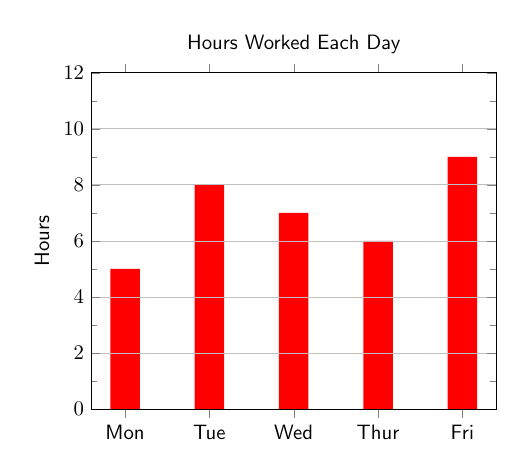
\begin{tikzpicture}[scale=0.75]
\begin{axis}[
ybar, axis on top, title={Hours Worked Each Day}, bar width = 0.5cm, ymajorgrids,
ymin = 0, ymax = 12, ylabel = {Hours},
symbolic x coords = {Mon, Tue, Wed, Thur, Fri}, xtick=data, minor y tick num = 1
]
\addplot [draw=none, fill=red] coordinates{
	(Mon,5) (Tue,8) (Wed,7) (Thur,6) (Fri,9)
};
\end{axis}
\end{tikzpicture}
\end{center}

\newpage 

\textsc{Clustered Bar Graph:}
\begin{center}
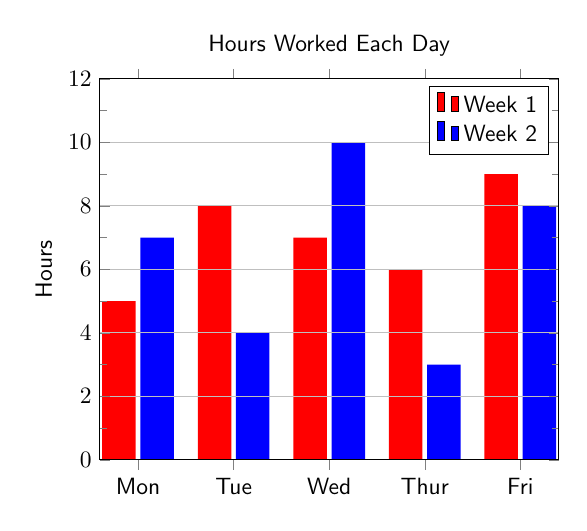
\begin{tikzpicture}[scale=0.85]
\begin{axis}[
ybar, axis on top, title={Hours Worked Each Day}, bar width = 0.5cm, ymajorgrids,
ymin = 0, ymax = 12, ylabel = {Hours}, legend entries = {Week 1, Week 2},
symbolic x coords = {Mon, Tue, Wed, Thur, Fri}, xtick=data, minor y tick num = 1
]
\addplot [draw=none, fill=red] coordinates{
	(Mon,5) (Tue,8) (Wed,7) (Thur,6) (Fri,9)
};
\addplot [draw=none, fill=blue] coordinates{
	(Mon,7) (Tue,4) (Wed,10) (Thur,3) (Fri,8)
};
\end{axis}
\end{tikzpicture}
\end{center}

\vfill 

\textsc{Stacked Bar Graph:}
\begin{center}
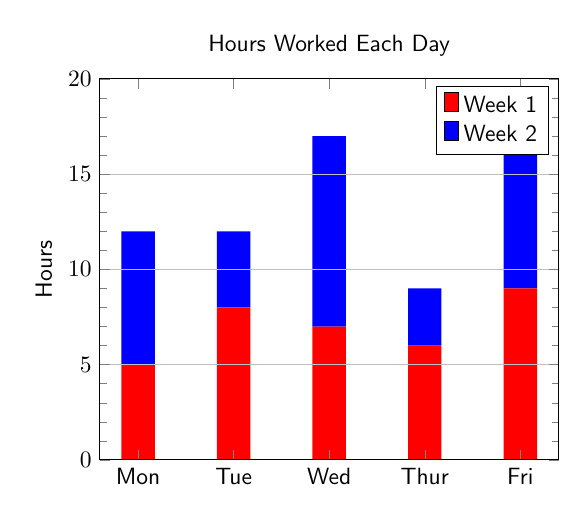
\begin{tikzpicture}[scale=0.85]
\begin{axis}[
ybar stacked, axis on top, title={Hours Worked Each Day}, bar width = 0.5cm, ymajorgrids,
ymin = 0, ymax = 20, ylabel = {Hours}, legend entries = {Week 1, Week 2},
symbolic x coords = {Mon, Tue, Wed, Thur, Fri}, xtick=data, minor y tick num = 4
]
\addplot [draw=none, fill=red] coordinates{
	(Mon,5) (Tue,8) (Wed,7) (Thur,6) (Fri,9)
};
\addplot [draw=none, fill=blue] coordinates{
	(Mon,7) (Tue,4) (Wed,10) (Thur,3) (Fri,8)
};
\end{axis}
\end{tikzpicture}
\end{center}

\vfill 

\textsc{Horizontal Bar Graph}
\begin{center}
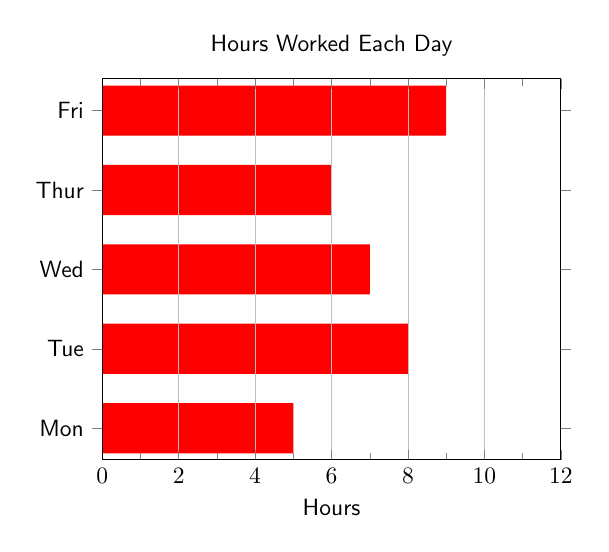
\begin{tikzpicture}[scale=0.85]
\begin{axis}[
xbar, axis on top, title={Hours Worked Each Day}, bar width = 0.75cm, xmajorgrids,
xmin = 0, xmax = 12, xlabel = {Hours},
symbolic y coords = {Mon, Tue, Wed, Thur, Fri}, ytick=data, minor x tick num = 1
]
\addplot [draw=none, fill=red] coordinates{
	(5,Mon) (8,Tue) (7,Wed) (6,Thur) (9,Fri)
};
\end{axis}
\end{tikzpicture}
\end{center}

\vfill 
\newpage 

\textsc{Relative Frequency (Percent of Total)}
\begin{center}
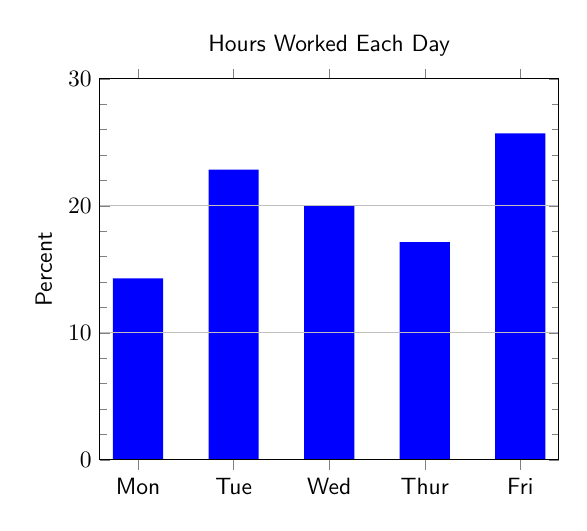
\begin{tikzpicture}[scale=0.85]
\begin{axis}[
ybar, axis on top, title={Hours Worked Each Day}, bar width = 0.75cm, ymajorgrids,
ymin = 0, ymax = 30, ylabel = {Percent}, minor y tick num = 4,
symbolic x coords = {Mon, Tue, Wed, Thur, Fri}, xtick=data
]
\addplot [draw=none, fill=blue] coordinates{
	(Mon,14.29) (Tue,22.86) (Wed,20) (Thur,17.14) (Fri,25.71)
};
\end{axis}
\end{tikzpicture}
\end{center}
\vspace{0.5in}

\subsubsection*{Creating a Bar Graph}

\begin{itemize}
    \item Create a frequency chart
    \item Displays count (or relative count) of each observation
\end{itemize}

\begin{center}
\begin{tabular}{c|c|c}
\textbf{Day} & \textbf{Hours Worked} & \textbf{Percent Total} \\ \hline
Monday 		& 	5	&	14.29\%	\\
Tuesday 	& 	8	&	22.86\%	\\
Wednesday	&	7	&	20.00\%	\\
Thursday	&	6	&	17.14\%	\\
Friday		&	9	&	25.71\%	\\
\end{tabular}
\end{center}
\vspace{1in}

\begin{example}
One week, a questionnaire was given to hotel guests asking them to rate their satisfaction with their experience. The ratings ranged from 1 (not satisfied) to 5 (very satisfied). Construct a bar graph of the data below:	\newline\\
\begin{tabular}{cccccc}
2&3&1&2&3&4\\
1&5&5&2&2&4\\
5&3&2&5&3&4\\
4&3&5&1&1&1\\
3&5&3&1&4&5
\end{tabular}
\end{example}

\vfill 
\newpage 

\begin{example}
Construct a relative frequency bar graph of the hotel ratings.
\end{example}
\vfill 

\begin{example}
Seeing the results of the questionnaires, the hotel made some changes and the following month, asked 40 new guests to rate their experience. The results, along with the previous results are listed:	\newline\\
\begin{center}
\begin{tabular}{c|c|c}
\textbf{Rating} & \textbf{Frequency (Sample 1)} & \textbf{Frequency (Sample 2)} \\ \hline
One & 6 & 4 \\
Two & 5 & 3 \\
Three & 7 & 12 \\
Four & 5 & 10 \\
Five & 7 & 12 
\end{tabular}
\end{center}
Construct a stacked bar graph of the results.
\end{example}

\vfill 
\newpage 

\begin{example}
Given the bar graph below, find the percent of people who travel in the summer.   
\vspace{0.25in}

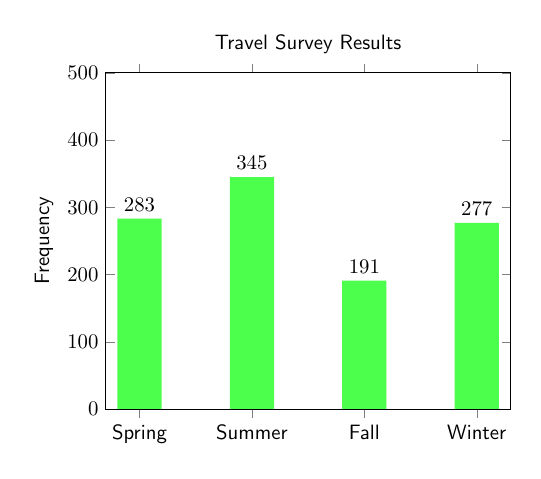
\begin{tikzpicture}[scale=0.75]
\begin{axis}[
ybar, axis on top, title={Travel Survey Results}, bar width = 0.75cm,
ymin = 0, ymax = 500, ylabel = {Frequency},
symbolic x coords = {Spring, Summer, Fall, Winter}, xtick=data, nodes near coords
]
\addplot [draw=none, fill=green!70] coordinates{
	(Spring,283) (Summer,345) (Fall,191) (Winter,277)
};
\end{axis}
\end{tikzpicture}
\end{example}

\vfill 

\subsection*{Pie Charts}

\begin{itemize}
    \item Allow for quick comparison of the part-to-whole nature of percentage. 
    \item Each slice of the pie (the central angle) is proportional to the percentage that slice is of the whole.
    \item Related to a pie chart is a \textit{donut chart}
\end{itemize}

\vfill 

\begin{example}
The pie chart below represents the hours worked each day as a percentage of the week. What total percent of the week was spent working on Monday and Tuesday?	\vspace{0.25in}

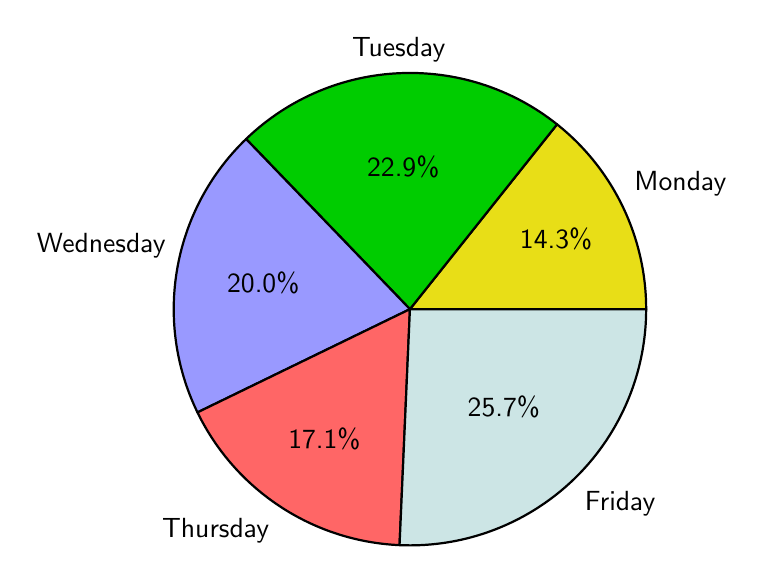
\begin{tikzpicture}
\pie[color = {
        yellow!90!black,
        green!80!black,
        blue!40, 
        red!60,
        teal!20}]{
14.3/Monday,
22.9/Tuesday,
20.0/Wednesday,
17.1/Thursday,
25.7/Friday
}
\end{tikzpicture}
\end{example}

\vfill 

\end{document}
